%\setlength{\epigraphwidth}{0.5\textwidth}
%\epigraph{There is an art in the contemplation of water. It is necessary to look at it as foaming in waves.}{--- \textup{Mencius}, \textit{\\translated by James Legge}}

The SNO+ water phase data were taken from May 2017 to September 2018. The period from May 2017 to October 2018 is the first stage of the water phase. During this stage, several calibration runs were taken, including the $^{16}$N calibration scans and the laserball scans. During the period from October 2018 to July 2019, over 20 tonnes of LAB (without PPO) was filled into the detector and the LAB mostly occupied the neck volume, slightly below the neck bottom. With the nitrogen cover gas on the top of the AV, the dataset taken during this period is called ``low background dataset''. 

In this chapter, I applied the MPW reconstruction algorithm mentioned in Chapter 4 as a position and direction fitter to the raw dataset as well as the run-by-run simulations. The fitted event vertex was used by the energy fitter developed by the SNO+ collaboration.  

I mainly analyzed the low background dataset. 

\section{Detector Backgrounds}

\subsection{Physics Backgrounds}

Radioactive Isotopes

assays


in-situ
ex-situ

the instrumental backgrounds can be removed by the data-cleaning approaches.



\subsection{Instrumental Backgrounds}

\section{High Level Cuts: Classifiers}

A set of classifiers have been developed since the SNO analysis and been optimized for the SNO+ data \cite{highlevel}.


\begin{itemize}

\item[$\bullet$] In time ratio (ITR) classifier

This classifier calculates the ratio of the number of hits in an optimized prompt time window ([-2.5,5.0]~ns for the water phase) to the total number of hits.


\item[$\bullet$] $\beta_{14}$ isotropy classifier

This classifier uses Legendre polynomials to return the	first ($\beta_1$) and the fourth ($\beta_4$) spherical	harmonics of an event, where:
\[
\beta_l = \frac{2}{N(N-1)}\sum_{i=1}^{N-1}\sum_{j=i+1}^N P_l(\cos\theta_{ij})
\]
and $P_l(\cos\theta_{ij})$ are Legendre polynomials.

The	combination	of these two polynomials returned by the classifier	was	
practically	chosen by the SNO collaboration	to be: $\beta_{14}=\beta_1+4\beta_4$
as	this gives	something that looks kinda gaussian-like	for	Cherenkov	events.	
Essentially	any	deviation from zero suggests some polarity (i.e. the event is not isotropic).	


\item[$\bullet$] $\theta_{ij}$ isotropy classifier 

describes the angle subtended at an event vertex by PMT \#i and PMT \#j.

\[
\cos\theta_{ij}=\frac{(\vec{X}_{PMT\#i}- \vec{X}_{event})\cdot (\vec{X}_{PMT\#j}- \vec{X}_{event})}{|\vec{X}_{PMT\#i}- \vec{X}_{event}||\vec{X}_{PMT\#j}- \vec{X}_{event}|}
\]
\end{itemize}

\subsubsection{Open Dataset Analysis}

MPW fit results

fiducial volume cut effects

\begin{table}[ht]
	\centering
	\caption{Candidate events in the open dataset. Compared the fitted results of the candidate events with different fitters.}
	\label{opendata}
	\begin{tabular*}{150mm}{c@{\extracolsep{\fill}}cccccccc}
		\toprule
	 Fitter &	Run &  GTID &  $z-0.108$(m) & $R$(m)& $(R/R_{av})^3$ & $\cos\theta_{sun}$ & SNO+ Day\\
		\hline 
	Rat & 100093 &11108354 &3.49 &3.57 &0.21 &-0.954459 &2683.92 \\	
	MPW &  --& --& 3.43 &	3.52 &	0.20	& -0.906388 & --\\
	Rat &	100207 &5079885 &-2.61 &4.60 &0.45 &0.816215 &2687.04\\
	MPW &	 --& --& -3.63 & \textbf{7.61} &	2.03 & \textbf{0.656374} & -- \\
	Rat &100632 &7882360 &1.77 &3.19 &0.15 &0.937212 &2696.93\\
	 MPW &    --& --&  1.67 & 3.11 &	0.14 & 0.910527 & -- \\
	Rat &100663 &15767175 &-4.33& 4.96 &0.56 &0.977517 &2698.18\\
	MPW & --& -- &-4.45 &	5.07 &	0.60 &	0.979943 & -- \\
	Rat &100915 &169700 &-1.00 &5.10 &0.61 &0.341287 &2701.23\\
	MPW &	--& --& -1.08 &	5.08 &	0.61 &	0.336706 & -- \\	
		\bottomrule
	\end{tabular*}
\end{table}

\begin{table}[ht]
	\centering
	\caption{Candidate events in the open dataset, searched by the MPW fitter.}
	\label{opendataMPW}
	\begin{tabular*}{150mm}{c@{\extracolsep{\fill}}cccccccc}
		\toprule
		Run & GTID & energy & $z-0.108$ & $R$ & $(R/R_{av})^3$ & $\cos\theta_{sun}$\\
		\hline 
100093 &	11108354	&5.827 & 3.43 & 3.52 & 0.20 & -0.907005\\
100632&	7882360    &6.183& 1.67 &3.11 &0.14 &0.9146124\\
100663&	15767175   &	6.182 & -4.45 &5.07 &0.60&	0.9807349\\
100915&	169700   &	5.684 &	-1.07 &5.08 &0.61&0.3385341\\
100984&	8621621&	5.701 & 0.76 &4.75 &0.502&-0.647735\\
101075&	11673714&	5.667 &4.43 &5.18 &0.64& 0.5873025\\

		\bottomrule
\end{tabular*}
\end{table}

In SNO+ water phase, solar $\nu_e$s are basically measured via elastic scattering $\nu_e+e^-\to \nu_e+e^-$. The maximum kinetic energy of the recoil electron is
$T_{max}=\frac{2E^2_\nu}{2E_\nu+m_e c^2}$
the cross section is $\sigma(\nu_e+e^-\to \nu_e+e^-)=9.52\times 10^{-44}(E_\nu/10~MeV)~cm^2$
the expected solar neutrino rate is 
$R=A\int_{T_{thresh}}^{T_{max}}\frac{d\sigma}{dE}\frac{dN}{dE_\nu}dE_\nu$.

A ``solar angle'', $\theta_{sun}$ is the direction of the event relative to the Sun's location,
$\cos\theta_{sun}\equiv \vec u_{event}\cdot (\vec{X}_{event}-\vec{X}_{sun})$, where $\vec{X}_{event}-\vec{X}_{sun}$ can be replaced by the Sun's location relative to the SNOLAB location since the whole lab can be treated as a point regarding the long distance to the Sun.


\subsection{TMVA Analysis}

The Toolkit for Multivariate Data Analysis with ROOT (TMVA) \cite{tmvaWebsite,albertsson2007tmva}

Boosted Decision Tree (BDT) method is used for the multiple variable analysis (MVA).

Receiver Operating Characteristic (ROC) curve describes the signal/background binary classifier system.

The MC simulations of the realistic runs (200004 to 207718) were used.
Different types of MC simulations were merged into a mixed dataset. Table.~\ref{table:mixed_MC} summarizes the types of simulations.

\begin{table}[ht]
	\centering
	\caption{Datasets of MC simulations.}
	\label{table:mixed_MC}
	\begin{tabular*}{150mm}{c@{\extracolsep{\fill}}cccccccc}
		\toprule
		Simulations & Simulated positions in the detector\\
		\hline 
        $^{208}$Tl & inner AV (internal $^{208}$Tl)\\
        -- & AV \\
        -- & external water (external $^{208}$Tl)\\
         $^{214}$Bi & inner AV (internal $^{214}$Bi)\\
        -- & AV \\
        -- & external water (external $^{214}$Bi)\\
        Solar $\nu_e$ & inner AV (internal $\nu_e$)\\
        -- & AV \\
        -- & external water (external $\nu_e$)\\
		\bottomrule
	\end{tabular*}
\end{table}


the simulated solar $\nu_e$ events are tagged as signals and mixed with $^{214}$Bi background events. The total dataset was divided into training and testing sets.
 tested. 









with discrimination threshold values. 

Area Under Curve (AUC)% 0.92
%energy cuts combining with NHit cuts


%6 variables used as inputs

%itr, $\theta_{ij}$, $\beta_{14}$, $NHits$, energy and $\hat u \cdot \hat R$.

MC simulations 

solar $\nu_e$ 
and $^{214}$Bi backgrounds

The distribution of $\cos\theta_{sun}$

\begin{figure}[!htb]
	\centering
	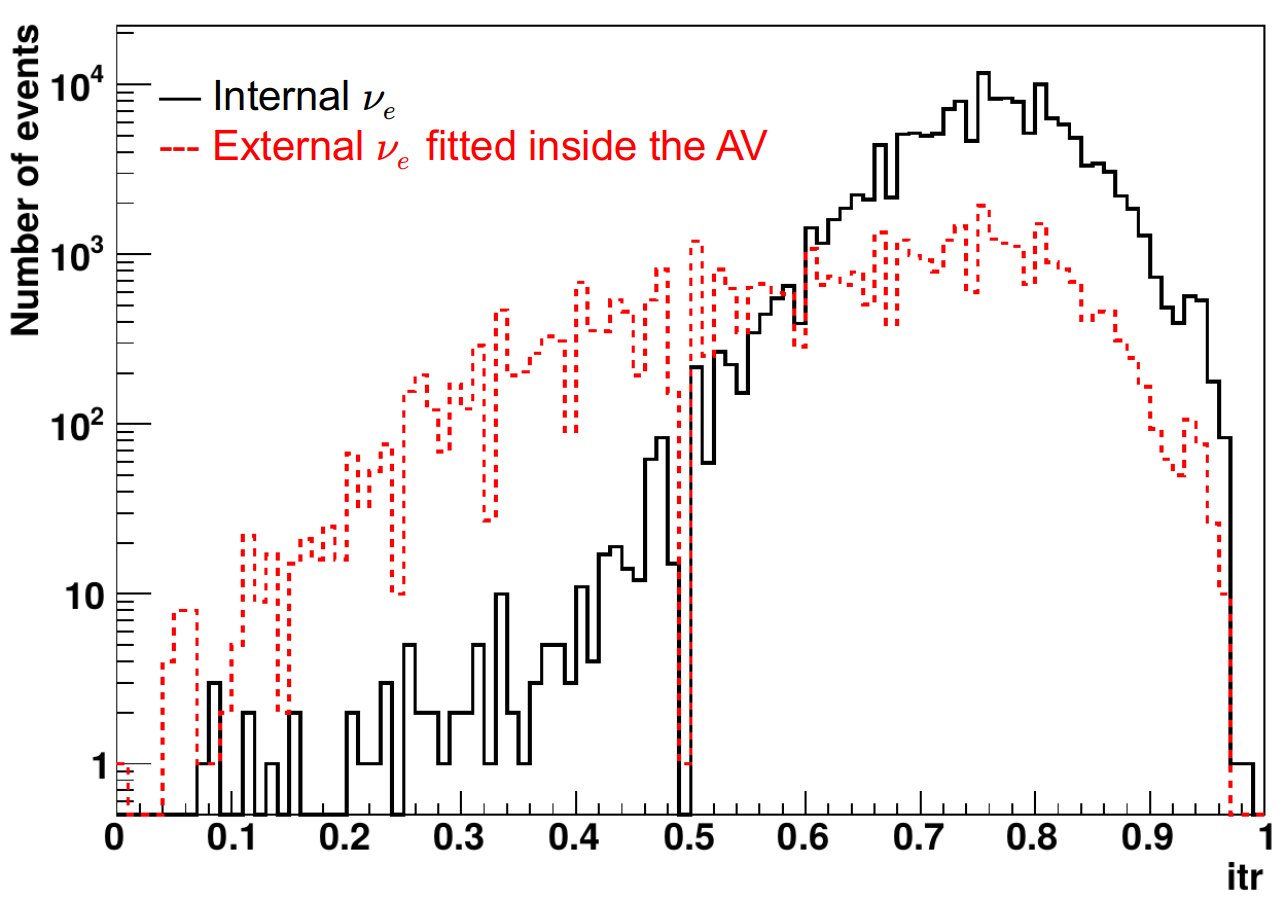
\includegraphics[width=8cm]{ITR_MPW_solarNuVsExSolar.png}
	\caption{Comparison between solar $\nu_e$ and external solar $\nu_e$; MPW results.}
	\label{itrCmp}
\end{figure}




Other packages developed for high energy particle physics, such as StatPatternRecognition (SPR)\cite{sprWebsite}, can be considered as an alternative tool or as a reference for results comparisons. 


\subsection{Likelihood Fits for Solar Neutrino Candidate Events}


